\documentclass[11pt, oneside]{article}   	% use "amsart" instead of "article" for AMSLaTeX format
\usepackage{geometry}                		% See geometry.pdf to learn the layout options. There are lots.
\geometry{letterpaper}                   		% ... or a4paper or a5paper or ... 
\usepackage{graphicx}				% Use pdf, png, jpg, or eps§ with pdflatex; use eps in DVI mode
								% TeX will automatically convert eps --> pdf in pdflatex		
\usepackage{amssymb}
\usepackage{mhchem}


\date{}							% Activate to display a given date or no date
\parindent 0in
\parskip 6pt


 
\begin{document}

\title{\bf Transient Groundwater Flow}
\maketitle
 
\section*{Overview and Learning Goals}
In this lecture you will learn about a numerical solution for the one-dimensional (1D), transient, groundwater flow problem for a homogeneous confined aquifer.  In particular, you will learn:
\begin{itemize}
\item How to discretize a 1D model into finite width cells
\item How to use the finite difference method to  numerically approximate 1st and 2nd order derivatives in space and time
\item About the  diffusion equation that governs  transient groundwater flow
\item How to solve the transient groundwater flow problem in 1D using explicit time stepping and the incorporation of boundary conditions.
\end{itemize}

%------------------------------------------------------------------------------------------
\section*{Background: The Finite Difference Method}
%------------------------------------------------------------------------------------------
 The finite difference method is a numerical technique for approximating the derivatives that are found in differential equations.  It is one of the main techniques (along with the finite element and finite volume methods) that is used to solve partial differential equations in the physical sciences. Other common methods include the finite element method and the finite volume method, however, the finite difference technique is probably the simplest and most straightforward  of these.
 
 The finite difference approximation for a first order derivative of a function at the location $x_0$ can be derived from a Taylor series expansion of a function:
 \begin{eqnarray}
f(x_0 + \Delta x) = f(x_0) + \frac{f'(x_0)}{1!} \Delta x + \frac{f''(x_0)}{2!}\Delta x^2 + ...
\end{eqnarray}
Rearranging this equation so that the first order derivative is on the left hand side gives:
\begin{eqnarray}
f'(x_0) = \frac{f(x_0 + \Delta x) - f(x_0)}{\Delta x} - \frac{f''(x_0)}{2!} \Delta x + ...
\end{eqnarray}
This equation shows that  the derivative of the function at $x_0$ can be approximated from the difference of the function values at $x_0+ \Delta x$ and at $x_0$.   The last term on the right hand side of the equal sign can be made negligible by choosing a very small value for $\Delta x$, which is the distance between the points. This allows the derivative to be simply approximated using only the first term on the right hand side. It can help to visualize this by imaging a plot of a relatively simple smooth function; pick two points on the curve that are close by. The difference of the function value at these two points, normalized by the spacing between them, will be close the derivative of the function. As you make the two points closer and closer together, this normalized difference will asymptotically approach the value of the functions's derivative.
 
This is the basis of the finite difference method. You simply approximate the derivatives in a partial differential equation by differencing nearby values of the function. We will see how this works later on here when we consider the groundwater flow equation.

We can state the finite difference formula for a grid of $n$ values of $x = \{x_0, x_1, x_2, x_3, ... x_n\}$ with grid spacing $\Delta x$ as:
\begin{eqnarray}
f'(x_i) \approx \frac{f(x_{i+1}) - f(x_i)}{\Delta x} 
\label{FOFD}
\end{eqnarray}
This is known as a forward finite difference formula since the function is evaluated at the present location $x_i$ as well as the next forward location $x_{i+1}$. There are other first order derivative formulas for backward and central differences, but we will not consider them here.

A similar method is used to find the formula for the second order derivative approximation. We will skip the derivation and just state the formula:
\begin{eqnarray}
f''(x_i) \approx \frac{f(x_{i+1}) - 2 f(x_i) + f(x_{i-1})  }{\Delta x^2} 
\label{SOFD}
\end{eqnarray}
This is known as a central finite difference method since it uses the function  values on the right side at $x_{i+1}$ and left side at $x_{i-1}$, in addition to the central value at $x_i$.

Note that while the examples above  looked at the finite difference formulas for a function of spatial position $x$, they also apply to functions of other variables such as time $t$. In the transient groundwater problem below, you will use finite difference formulas for both position $x$ and time $t$.

%------------------------------------------------------------------------------------------
\section*{One-Dimensional Groundwater Aquifer Model}
%------------------------------------------------------------------------------------------
Before we get to the modeling problem, we need to introduce some definitions that will be used in our model setup. 

 \begin{description}
\item[aquifer ] A geological unit consisting of fractured rocks or a bed of grains that can both store and transmit water.
\item[groundwater flow ]  Fluid moves through an aquifer by transmission through the pore spaces between  grains  This is also sometimes  referred to a porous flow. Fluid can also move  through  fractures in a  rock formation.  
\item[hydraulic head, $h$   ]  This is a combination of both the elevation head $z$ (with units meters), which is the height of the water relative to some datum (such as sea level), as well as the pressure head, $\psi$ which is the height the water would obtains above the elevation head due to pressure ($\psi = P/\rho g$, where $P$ is pressure, $\rho$ is density, and $g$ is gravitational acceleration).  Thus we have $h = z + \psi$.

Hydraulic head is a useful quantity for determining where water will flow (or not), since water will only flow from areas of high  to low hydraulic head. For example, water flows downhill since the head decreases. Water in  a spigot connected to the bottom of a water jug flows out since the head outside the water jug is less than that on the inside of the jug.
\end{description}

For our 1D aquifer model, we define the following properties:
\begin{description}
\item[thickness $b$  {\rm [m]}]  The thickness of the aquifer unit in meters.
\item[hydraulic conductivity $K$ {\rm [m/s]} ]  The ease which which water can move through the pore spaces or fractures in the aquifer.  $K$ depends primarily on the permeability of the aquifer and the degree of saturation, but also the viscosity and permeability of the fluid.
\item [specific storage $S_s$ {\rm [m$^{-1}$]}] This property defines how much water the particular rock type can hold. It depends primarily on the porosity of the rock (i.e., how much empty space is there between grains). It is  the mass of water that an aquifer releases per mass of aquifer, per unit decline in hydraulic head.
\end{description}

While $K$ and $S_s$ are properties that primarily are determined by the rock type, there are two related parameters that are formed by integrating these properties over the thickness of the aquifer $b$:

\begin{description}
\item[transmissivity $T$ {\rm [m$^2$/s]} ]  $T = K b$. This is similar to hydraulic conductivity but includes the aquifer thickness.  Transmissivity is a measure of how much water can be transmitted horizontally.
\item [storativity $S$ {\rm [unitless]}] $S = S_s b$.  This is similar to the specific storage but  includes the aquifer thickness. Storativity is the volume of water released from aquifer per unit decline in hydraulic head, per unit area of the aquifer.
\end{description}



\begin{figure}[htbp]
\begin{center}
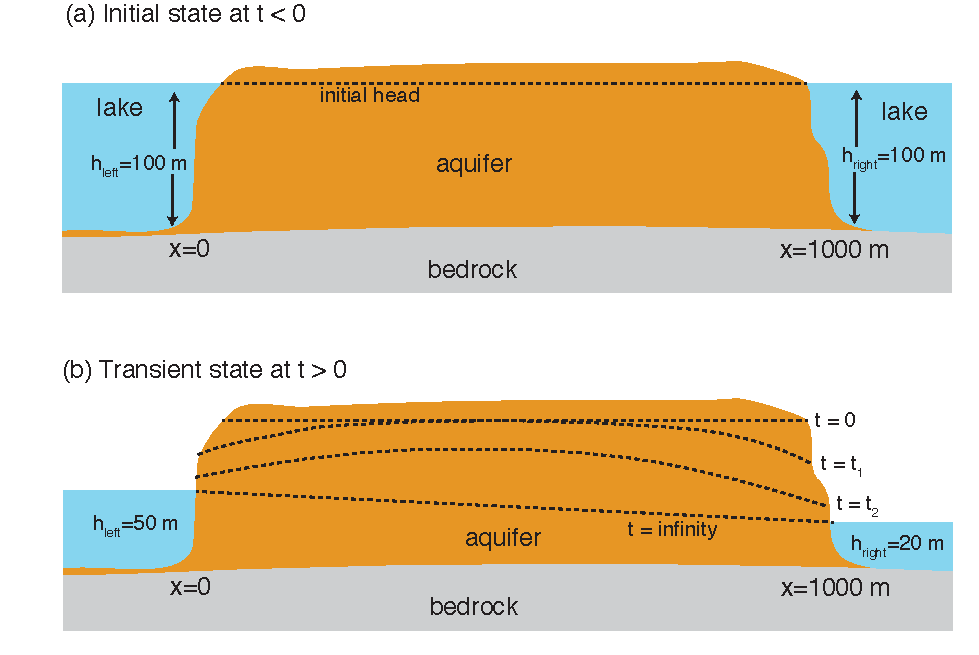
\includegraphics[width=.75\textwidth]{aquifer_model.pdf}
\caption{Groundwater aquifer model problem setup at (a) the initial state when $t<0$ and (b) at $t>0$ after a rapid change in the lake depths.     }
\label{model}
\end{center}
\end{figure}

The upper panel in Figure \ref{model} shows the initial state of the 1D model. The aquifer is 1000 m long and 100 m thick (here the aquifer is unconfined). Prior to the start of the model ($t < 0$), head in the aquifer was fixed by boundaries on either side, a lake to the left and a lake to the right. Boundary heads were such that head in the aquifer was constant, $h = 100$ m, so there was no flow in or out through the boundaries. At $t = 0$, head on both sides of the aquifer drops instantaneously, to 50 m on the left and 20 m on the right. We want to know how the head changes in the aquifer with time, from $t_0$ to $t_1$ to $t_2$ and so on until the head is no longer changing. 

We will assume the aquifer is unconfined, meaning there is no overlying confining layer. Further, we will assume the aquifer is homogeneous, meaning that $K$ and $S_s$ do not vary with position. The governing equation for flow in this one dimension homogeneous system is:
\begin{eqnarray}
\frac{T}{S} \frac{\partial^2 h}{\partial x^2} = \frac{\partial h}{\partial t},
\label{transient}
\end{eqnarray}
where $\partial$ is the partial derivative operator. This equation is known as the {\bf transient groundwater flow equation}. The derivation of this equation starts with Darcy's law and mass conservation equations; however, we will omit the derivation here due to the length of time required. This will allow us to instead concentrate on a finite difference numerical solution of the equation.

Before embarking on the numerical solution, it is always worthwhile to consider the various terms in the differential equation. The term on the left hand side of the equation is the second order spatial derivative of the hydraulic head $h$. In other words, this is the spatial curvature of the hydraulic head. $ \frac{\partial h}{\partial t}$ is the first order time derivative of  the hydraulic head. Thus we have a first order time derivative equal to some coefficients multiplying  a second order spatial derivative. This is known as a diffusion equation since it describes the diffusion of some quantity through space as a function of time.


You have likely already encountered a similar differential equation for heat flow, where $h$  is replaced by temperature and $S$ and $T$ are replaced by terms for heat capacity and thermal conductivity. For the groundwater flow equation considered here, the ratio $T/S$ is known as the hydraulic diffusivity.  If this ratio is large we can see that the time derivative of the hydraulic head will be large.  This makes sense from intuition: since $T$ is the transmissivity of the aquifer, it makes sense that the head will increase or decrease more quickly with $T$.  We can also see that the time changes in the hydraulic head will be largest where the spatial curvature of the head is largest.  {\it When you are looking at your results for the homework problem and possibly wondering if they are correct, consider this last point carefully, especially for the early time steps in the model.}

My last comment is that this differential equation is called a homogeneous equation since there are no terms for sources or sinks. For example, if we had a well where water was being extracted from the aquifer for drinking water or farm irrigation, or where water was being injected (say for waste disposal or hydraulic fracturing for oil exploration), the equation would need to include  additional terms to describe this sources and sinks, and then the equation would be called an inhomogeneous equation. 

%------------------------------------------------------------------------------------------
\section*{Finite Difference Numerical Solution}
%------------------------------------------------------------------------------------------

Now we will numerically approximate the solution to the partial differential equation (\ref{transient}) using the finite difference method.  Since this is a one-dimension problem, our modeling grid will consist of a 1D grid of cells arranged laterally as shown in Figure \ref{grid}.
%
\begin{figure}[tb]
\begin{center}
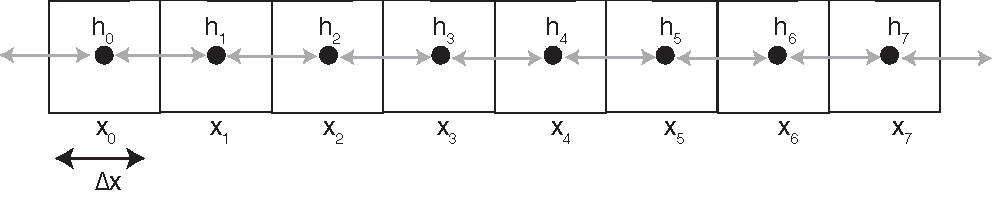
\includegraphics[width=.75\textwidth]{grid.pdf}
\caption{1D finite difference grid cells example.  The cells have spacing $\Delta x$ and gray arrows represent flow between cells. In our simple example, each cell has the same values for $T$, $S$ and $b$.  }
\label{grid}
\end{center}
\end{figure}
 
We will divide our problem up into evenly spaced cells of 25 m width, denoting the position of each cell as $x = \{x_0, x_1, x_2, x_3, ... x_n\}$.   Within each cell we will solve for the evolution of the hydraulic head over time using evenly spaced values of time $t = \{t_0, t_1, t_2, t_3, ... t_m\}$.  We will represent head at position $x_j$ time step $t_k$ using the notation $h_j^k$. 


The explicit, finite-difference approximation for equation (\ref{transient}) is:
\begin{eqnarray}
\frac{T}{S}\frac{h^k_{j+1}-2 h^k_{j} + h^k_{j-1} }{\Delta x^2} = \frac{h_j^{k+1}-h_j^k }{\Delta t},
\label{fdtransient}
\end{eqnarray}
where the superscript $k$ refers to the current time, and $k+1$ refers to the next time and subscript $j$ refers to the cell or node. Subscript $j+1$ indicates the cell to the right, and subscript $j-1$ indicates the cell to the left.  

Suppose that we have initial values for all values of $h$ at time $t_k$; in other words, we know $h_j^k$ for all values of $j$ like in Figure 1 (a). Equation \ref{fdtransient} can then be rearranged so that we can solve for the head at the next time step $t_{k+1}$:
\begin{eqnarray}
h_j^{k+1} = h_j^{k} \left ( 1 - \frac{2T\Delta t}{S\Delta x^2} \right) +  \frac{T\Delta t}{S\Delta x^2} \left( h_{j+1}^{k} + h_{j-1}^{k} \right)
\label{fdtransient_step}
\end{eqnarray}

In this formulation, everything on the right-hand side (RHS) of the equation is known, being based entirely on head values from the previous time step $t_k$. 
 Thus you can solve for each value of  $h_j^{k+1}$ based on the previous values of $h$ at that location ($h_j^{k}$),and  the previous values of $h$ in the cells to either side of that location ( $h_{j-1}^{k}$ and $h_{j+1}^{k}$ ).
 This equation also includes the constant aquifer properties $T$ and $S$, the cell width ($\Delta x$), and the length of the time-step ($\Delta t$). 

Note that  the constant terms in equation \ref{fdtransient_step} can be grouped together into constant coefficients $a$ and $b$,  allowing for a  simpler version of the equation:
\begin{eqnarray}
h_j^{k+1} &=&a\, h_j^{k}  + b \left( h_{j+1}^{k} + h_{j-1}^{k} \right),
\end{eqnarray}
where
\begin{eqnarray}
a&=&  1 - \frac{2T\Delta t}{S\Delta x^2}, \\
b &=&   \frac{T\Delta t}{S\Delta x^2}.
\end{eqnarray}
Figure \ref{grid_step} graphically shows how a grid cell is updated from time step $t_k$ to $t_{k+1}$ by multiplying its value by $a$ and then adding this to $b$ multiplied by the neighboring values of $h$ from time step $t_k$ (and not $t_{k+1}$).

\begin{figure}[htbp]
\begin{center}
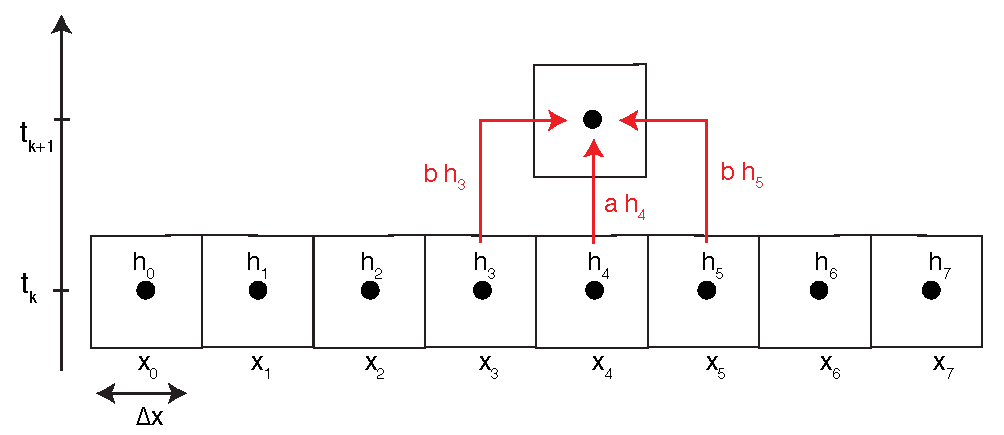
\includegraphics[width=.9\textwidth]{grid_step.pdf}
\caption{1D finite difference grid cells example.  The cells have spacing $\Delta x$ and gray arrows represent flow between cells. In our simple example, each cell has the same values for $T$, $S$ and $b$.  }
\label{grid_step}
\end{center}
\end{figure}

The time-step size should be limited by:
\begin{eqnarray}
 \frac{T\Delta t}{S\Delta x^2} \le 0.5
\end{eqnarray}
This ensures that the time step is small enough to be accurate using the finite difference approximation. Notice how it depends on both $T/S$ and $\Delta x^2$.


For this problem, you will not specify the number of time-steps you want the code to perform (i.e., you will not use a {\it for-loop}).  Instead, you will set up the code to continue stepping through time until some steady-state threshold has been reached, i.e., when the head $h$ is no longer changing appreciably between time-steps.  We will call this threshold our steady state tolerance, and define it to be equal to the sum of the absolute value of the differences in $h$ between the current and previous time-steps:
\begin{eqnarray}
\delta_h = \sum_j | h_j^{k+1} - h_j^k |
\end{eqnarray}
If the head is changing a lot between time steps, $\delta_h$ will be large, whereas once the solution is close to the steady state,  $\delta_h$ will become negligibly small.

Your homework assignment is to solve the transient groundwater equation using the finite difference method and the initial conditions shown in Figure 1(a) and (b). 

\end{document}  